\chapter{数据库设计}
\section{数据库环境说明}
本系统的数据系统采用MySQL数据库系统。

在服务器端采用Java编程语言,使用JDBC API。

\section{数据库的命名规则}
数据库的名字为BBDatabase。

数据表的命名规则为XX\_table,其中XX为数据表存储内容的英文单词,单词间用\_连接,首字母大写,如果英文单词长度大于5则使用缩写。

如HomeWork缩写为HW,Information缩写为Info。

表中每一个字段以该字段代表含义的小写英文单词命名,缩写同上。字段不加前缀。

\section{逻辑设计}
\subsection{逻辑设计的E-R图}
\begin{figure}[H]
\centering
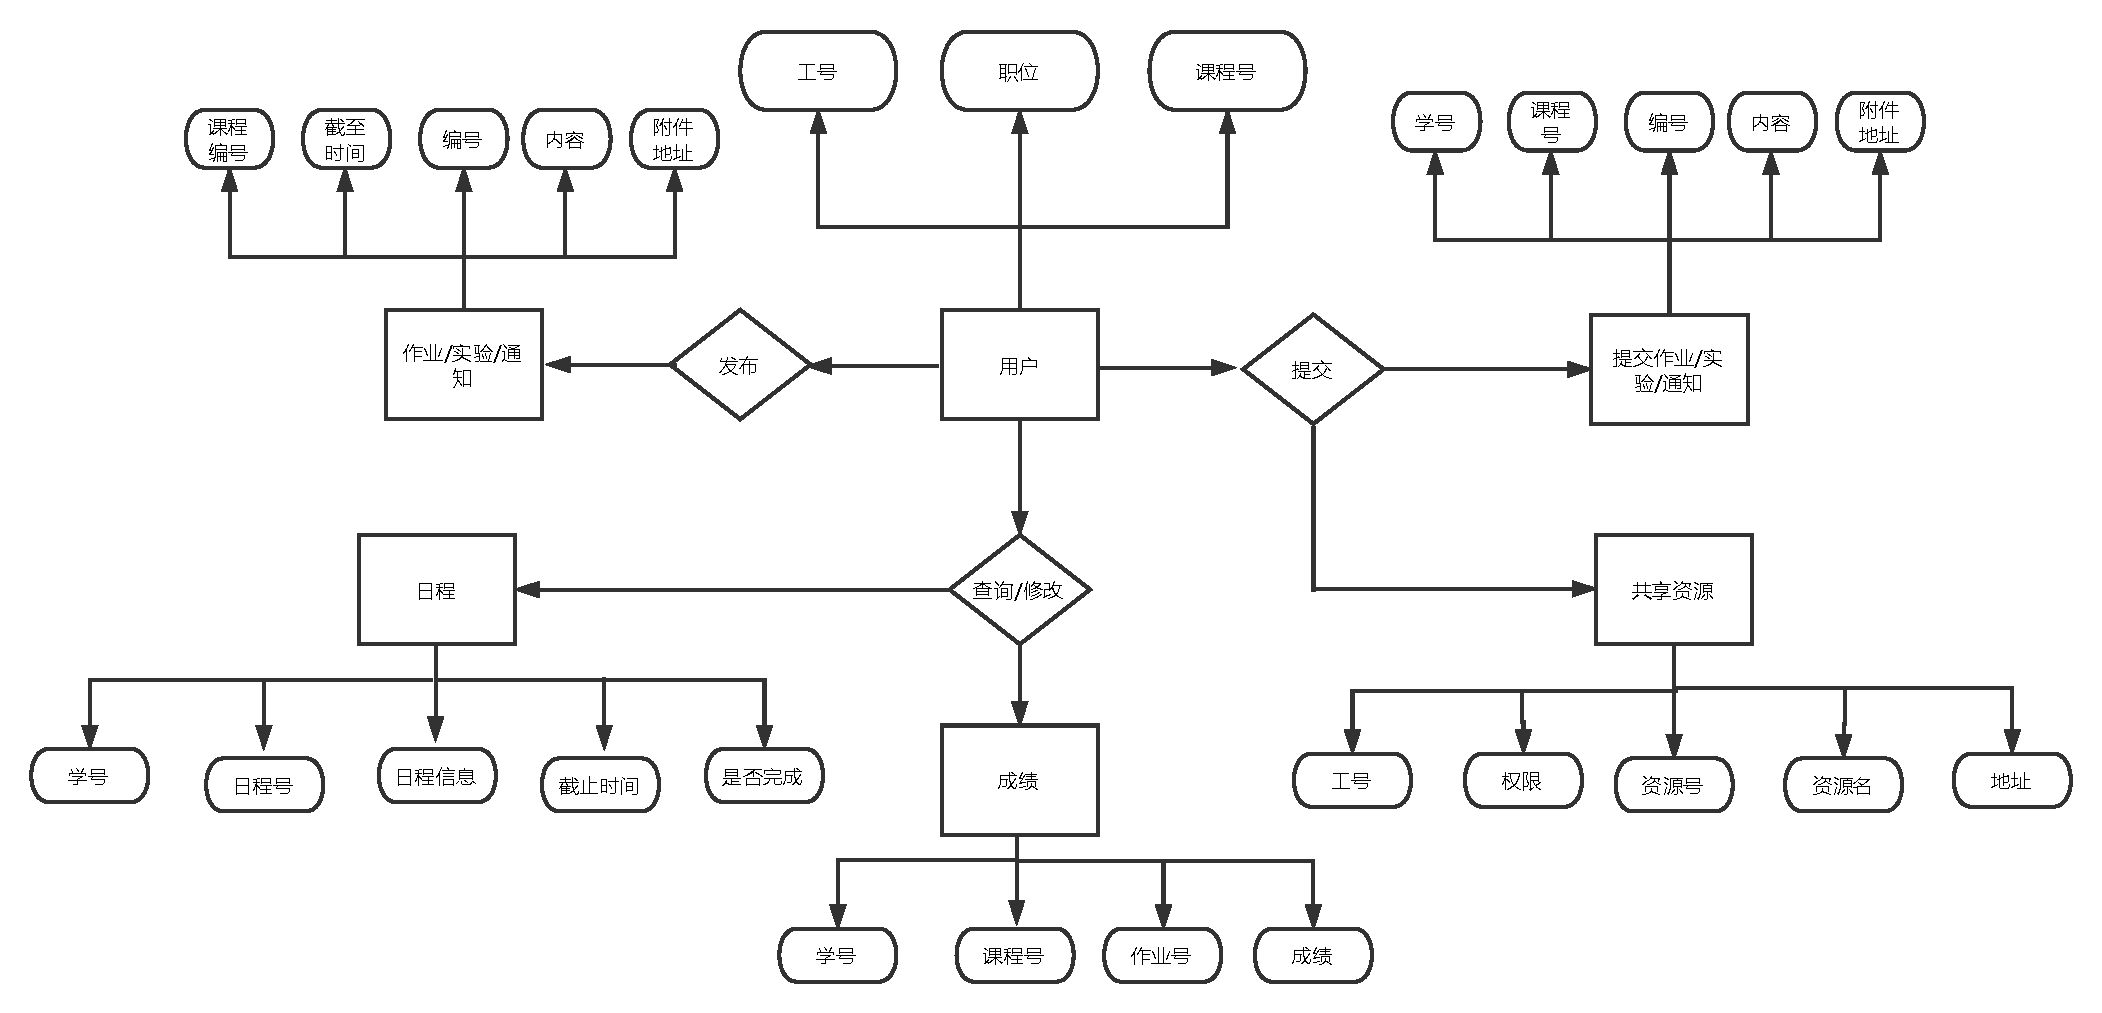
\includegraphics[width=15cm]{database}
\caption{数据库ER图}
\end{figure}

\section{物理设计}
\subsection{数据库产品}
使用Mysql数据库。

\subsection{实体属性、类型、精度}
\subsubsection{日程表:Sche\_table}

\begin{table}[htbp]
\centering
\caption{日程表} \label{tab:classification}
\begin{tabular}{|c|c|c|c|}
    \hline
    列名 & 数据类型 & 可否为空 & 说明 \\
    \hline
    UserID & Char & Not NULL & 用户学号 \\
    \hline
    ScheID & Int & Not NULL & 日程编号 \\
    \hline
    ScheInfo & VarChar & Not NULL & 日程内容 \\
    \hline
    DDL & Datetime & Not NULL & 截止日期 \\
    \hline
    Done & Bit & Not NULL & 是否完成 \\
    \hline
\end{tabular}
\end{table}
主键:\{UserID,ScheID\}


\subsubsection{作业/实验发布表: HW\_Pub\_table}

\begin{table}[htbp]
\centering
\caption{作业/实验发布表} \label{tab:classification}
\begin{tabular}{|c|c|c|c|}
    \hline
    列名 & 数据类型 & 可否为空 & 说明 \\
    \hline
    CourseID & Char & Not NULL & 课程编号 \\
    \hline
    HWID & Int & Not NULL & 作业编号 \\
    \hline
    HWInfo & VarChar & Not NULL & 作业内容 \\
    \hline
    DDL & Datetime & Not NULL & 截止日期 \\
    \hline
    AnnexAddr & VarChar & NULL & 附件地址 \\
    \hline
\end{tabular}
\end{table}
主键:\{CourseID,HWID\}


\subsubsection{作业/实验提交表: HW\_Sub\_table}

\begin{table}[htbp]
\centering
\caption{作业/实验提交表} \label{tab:classification}
\begin{tabular}{|c|c|c|c|}
    \hline
    列名 & 数据类型 & 可否为空 & 说明 \\
	\hline
    UserID & Char & Not NULL & 学号 \\
    \hline
    CourseID & Char & Not NULL & 课程编号 \\
    \hline
    HWID & Int & Not NULL & 作业编号 \\
    \hline
    HWInfo & VarChar & Not NULL & 提交内容 \\
    \hline
    AnnexAddr & VarChar & NULL & 附件地址 \\
    \hline
\end{tabular}
\end{table}
主键:\{UserID,CourseID,HWID\}


\subsubsection{用户信息表: User\_Info\_table}

\begin{table}[htbp]
\centering
\caption{用户信息表} \label{tab:classification}
\begin{tabular}{|c|c|c|c|}
    \hline
    列名 & 数据类型 & 可否为空 & 说明 \\
	\hline
    UserID & Char & Not NULL & 工号 \\
    \hline
    Position & Char & Not NULL & 职位 \\
    \hline
    CourseID & Char & NULL & 课程号 \\
    \hline
\end{tabular}
\end{table}
主键:\{UserID\}


\subsubsection{成绩表: Score\_table}

\begin{table}[htbp]
\centering
\caption{成绩表} \label{tab:classification}
\begin{tabular}{|c|c|c|c|}
    \hline
    列名 & 数据类型 & 可否为空 & 说明 \\
	\hline
    UserID & Char & Not NULL & 学号 \\
    \hline
    CourseID & Char & Not NULL & 课程号 \\
    \hline
    HWID & Int & Not NULL & 作业号 \\
    \hline
    Score & Int & Not NULL & 成绩 \\
    \hline
\end{tabular}
\end{table}
主键:\{UserID,CourseID,HWID\}


\subsubsection{笔记表: Note\_table}

\begin{table}[htbp]
\centering
\caption{笔记表} \label{tab:classification}
\begin{tabular}{|c|c|c|c|}
    \hline
    列名 & 数据类型 & 可否为空 & 说明 \\
	\hline
    UserID & Char & Not NULL & 学号 \\
    \hline
    NoteID & Int & Not NULL & 笔记号 \\
    \hline
    NoteName & VarCahr & Not NULL & 笔记名 \\
    \hline
    Note & VarChar & Not NULL & 笔记内容 \\
    \hline
\end{tabular}
\end{table}
主键:\{UserID,NoteID\}


\subsubsection{讨论区表: Note\_table}

\begin{table}[htbp]
\centering
\caption{讨论区表} \label{tab:classification}
\begin{tabular}{|c|c|c|c|}
    \hline
    列名 & 数据类型 & 可否为空 & 说明 \\
	\hline
    UserID & Char & Not NULL & 学号 \\
    \hline
    UserName & Char & Not NULL & 姓名 \\
    \hline
    ThemeName & VarCahr & Not NULL & 主题名 \\
    \hline
    ThemeAddr & VarChar & Not NULL & 主题地址 \\
    \hline
    ThemeTime & Datetime & Not NULL & 发布时间 \\
    \hline
\end{tabular}
\end{table}
主键:\{UserID,ThemeName\}


\subsubsection{资源共享表: Share\_table}

\begin{table}[htbp]
\centering
\caption{资源共享表} \label{tab:classification}
\begin{tabular}{|c|c|c|c|}
    \hline
    列名 & 数据类型 & 可否为空 & 说明 \\
	\hline
    UserID & Char & Not NULL & 工号 \\
    \hline
    UserAuth & Char & Not NULL & 权限 \\
    \hline
    Name & VarCahr & Not NULL & 资源名 \\
    \hline
    Addr & VarChar & Not NULL & 资源地址 \\
    \hline
    ResourceID & Int & Not NULL & 资源号 \\
    \hline
\end{tabular}
\end{table}
主键:\{UserID,ResourceID\}




\section{安全性设计}
管理默认用户:在生产环境中,必须严格管理 sys 和 system 用户,必须修改其默认密码,禁止用该用户建立数据库应用对象。删除或锁定数据库测试用户。

数据库级用户权限设计:必须按照应用需求,设计不同的用户访问权限。包括应用系统管理用户,普通用户等,按照业务需求建立不同的应用角色。用户访问另外的用户对象时,应该
通过创建同义词对象 synonym 进行访问。

角色与权限:确定每个角色对数据库表的操作权限,如创建、检索、更新、删除等。每个角色拥有刚好能够完成任务的权限,不多也不少。在应用时再为用户分配角色,则每个用户的权
限等于他所兼角色的权限之和。

应用级用户设计:应用级的用户帐号密码不能与数据库相同,防止用户直接操作数据库。用户只能用帐号登陆到应用软件,通过应用软件访问数据库,而没有其它途径操作数据库。
用户密码管理:用户帐号的密码必须进行加密处理,确保在任何地方的查询都不会出现密码的明文。

\section{数据库管理与维护说明}
对于数据库的维护,随时对数据库中的信息加以调试和保存备份。同样需要个工作人员进行系统的分析和用户的反馈,对系统进行升级以及功能的完善。同时保证系统安全有序的运行。
